\begin{figure}
  \centering
  \begin{subfigure}[b]{0.5\textwidth}
    \centering
    
\includegraphics[width=0.9\textwidth]{./img/raw/vp-perspectief/render.png}
    \caption{De render.}
    \label{fig:vp-perspectief:render}
  \end{subfigure}%
  \begin{subfigure}[b]{0.5\textwidth}
    \centering
    \begin{tikzpicture}
      \node[inner sep=0pt] (img1) at (0,0)
           {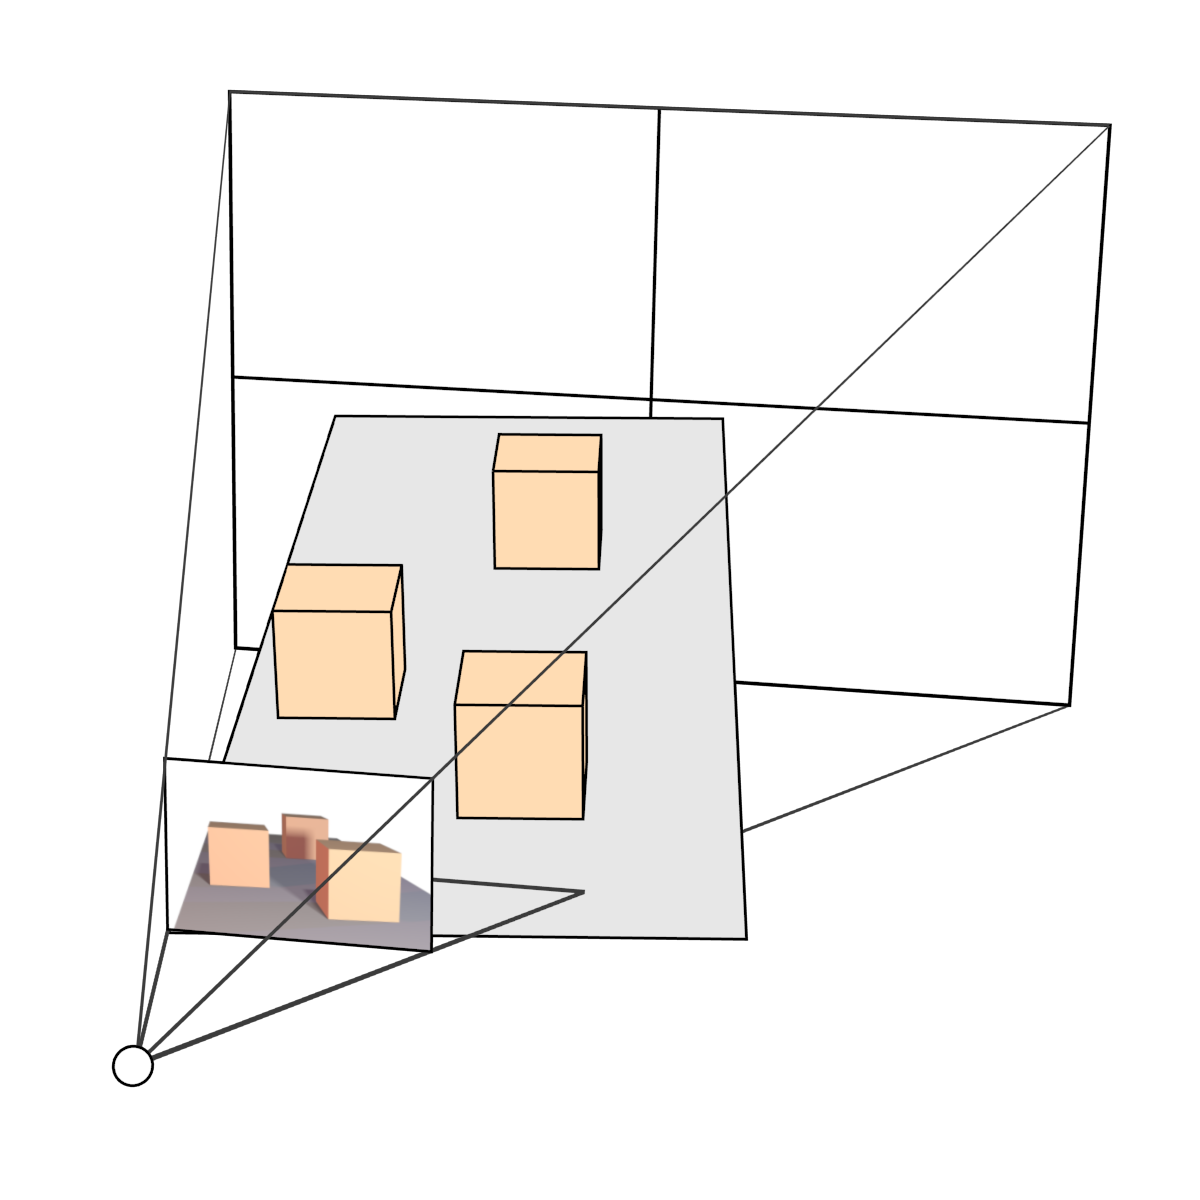
\includegraphics[width=\textwidth]{./img/raw/vp-perspectief/scene.png}};
      \node (camera) at (-0.23\textwidth,-0.41\textwidth) {Camera};
      \node (camera) at (0.0\textwidth,-0.35\textwidth) {Zichtvlak};
      \node (camera) at (0.42\textwidth,-0.135\textwidth) {Clipvlak};
    \end{tikzpicture}
    \caption{De scene.}
    \label{fig:vp-perspectief:scene}
  \end{subfigure}
  \caption{Perspectief projectie.}
  \label{fig:vp-perspectief}
\end{figure}
